\newpage
\section{Introduction}

\subsection{Laser Locking}

The ability to lock a laser to a very specific frequency is of great importance to the UBC Quantum Degenerate Gases Laboratory.  They use these optical systems to laser cool atomic and molecular gases.  This requires a very narrow linewidth on the laser, and a specific frequency.  Any improvement in the frequency precision of the laser will increase the quantity of atoms that can be trapped or cooled, as well as the attainable temperatures in a trap.  Often, this frequency must be very close to the natural transitions of the gas. \\

One way to acquire such a system is to pass the beam through a gas.  The gas has state transitions at particular optical frequencyes, which can be detected by sweeping the laser (or an associated probe beam).  When doing this, the gas atoms will absorb photons at the corresponding frequencies, which will appear on a spectrum analyser as in Figure XXXXX(Get a figure of the rubidium spectrum).  However, since the gas is at room temperature, the broad absorption dip will have a bandwidth of about 1 GHz, which is too wide for accurate laser locking.

\subsection{Doppler Effects}

Since the gas atoms are moving in different directions, some atoms will be moving towards the laser beam, and other atoms will be moving away from it (some will be in between, of course).  As a result, if a single laser is used, the atoms moving towards the laser will perceive a higher frequency, and thus will excite at lower frequencies than the resonance frequency.  The opposite is also true.  If the absorption-vs-frequency curve is measured for a laser passed through the gas, there is a wide smear that is approximately 1 GHz wide \cite{madison14}.  This makes the apparent spectrum of the gas much wider, and thus, much harder to lock a signal to.  This is depicted in Figure~\ref{fig:doppler}. \\

A major improvement is to redirect the single frequency laser around the sample, to the opposite side.  Now, when the sweep laser is at the same frequency as the pumping laser, its light will not be absorbed by the atoms with zero horizontal velocity.  This creates a Doppler-cancelled feature, which is about 10--100MHz wide.

\subsection{Acousto-Optic Modulator}

One way to modulate the frequency of the beam is to use an *acousto-optic modulator* (AOM)An AOM is a device that mechanically varies its shape, adjusting the distance the light has to travel to reach its destination.  By driving the optical medium at a particular frequency, an incident beam of light is diffracted and Doppler shifted depending on what angle it is sampled at. Modulating this driving frequency at an additional frequency $\Omega$, produces a beam of light that is phase modulated at a frequency $\Omega$. \\

AOMs are limited by the mechanical properties of the optical medium. Specifically, while
being driven at some nominal frequency that may reach up to 100s of MHz, they can only register a frequency modulation at a rate up to several MHz. This is due to the fact that the rate of acoustic propagation across the medium is limited. Depending on what refraction angle it is sampled at, the output beam of the acousto-optic modulator also contains a shift in the carrier frequency.  This shift needs to be accounted for in a later stage of the system.

\subsection{Electro-Optic Modulator}

An \emph{electro-optic modulator} (EOM), is a device that uses an electric field to modulate the phase of a light wave.  These devices exploit the effects of strong higher order susceptibility, whereby the speed of light in a crystal is affected by the presence of an electric field.  Therefore, by adjusting the electric field in the crystal, the phase (and ultimately frequency spectrum) of the beam can be varied.  The EOM does \emph{not} shift the carrier frequency, unlike an AOM. Furthermore, the resultant phase modulation frequency
of the incident laser can reach into the GHz range, orders of magnitude above the
capability of an AOM.\\

Unfortunately, the EOM requires fairly large driving voltages, on the order of hundreds of volts.  Some manufacturers provide a full EOM solution, with built-in amplifier, to make their equipment easier to use, making an external high-voltage amplifier unnecessary. This project makes use of a homebuilt EOM/driver system based around a LiNbO$_3$ crystal.

\subsection{The Pound-Drever-Hall Method}

Optical frequencies generally exceed 100THz. It is generally not possible to
extract information at these frequencies using conventional
electronic measurement equipment.  Systems make use of
schemes that down-mix these optical signals into RF range, which are then
processed via conventional means (RF electronics and digital systems). \\

The Pound-Drever-Hall method makes use of phase-modulated light to measure an
optical response and down-mix it into RF range.  This signal is then mixed again with the same oscillator to produce a DC signal. Changing the modulation frequency varies the resolution of this derivative function.  At extremes, this derivative function is either small and featureless, or is excessively noisy and not useful. \\

This method is used to lock to extrema of absorption spectra.  In an atomic gas, these features are typically transition and crossover resonances \cite{maguire2006}. Carefully selecting a modulation frequency to obtain a useful error signal about a point of interest is a principal challenge of implementing this method.

\subsection{Spectroscopy Methods}

Add a more well thought out paragraph about modulation transfer spectroscopy and maybe a figure to illustrate it. We should simply mention here how we were originally going to use saturated absorption spectroscopy but due to AM pickup, generally crappy SNR, we switched over to mod-transfer. We should include some pictures of saturated absorption signals.

% \begin{figure}
%     \centering
%     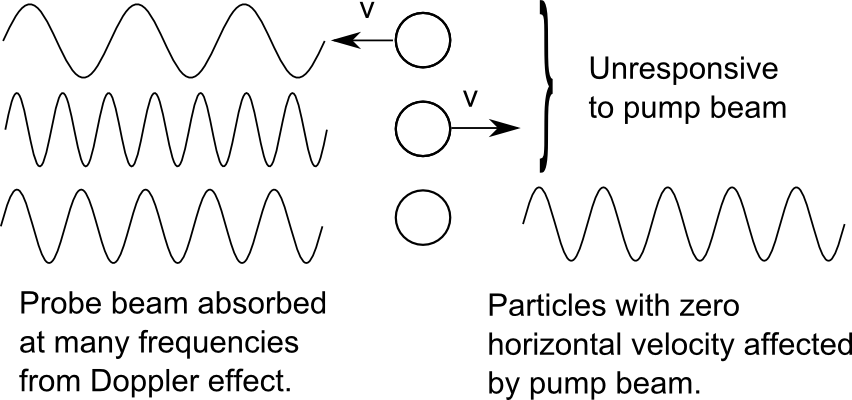
\includegraphics[width=9cm]{doppler.pdf}
%     \caption{Doppler effect demonstration.  Probe beam is absorbed across a wide frequency range, but only the non-Doppler-shifted particles are affected by both beams from left and right.}
%     \label{fig:doppler}
% \end{figure}

\begin{figure}
  \begin{tabular}{cc}
    \includegraphics[width=0.47\textwidth]{figures/{AOM_85}.png} &
    \includegraphics[width=0.47\textwidth]{figures/{AOM_87}.png} \\
  \end{tabular}
  \caption{something something danger zone}
\end{figure}
